
\begin{tikzpicture}
[
	scale=1,
	every node/.style={font=\sffamily\scriptsize},
	a/.style={
		-{Stealth[scale=1]},
		dashed,
		thick,
		rounded corners,
	},
	ia/.style={
		a,
		color=uniblue1,
	},
	la/.style={
		a,
		color=unired1,
	},
	asmol/.style={
		-{Stealth},
		dashed,
%		thick,
		rounded corners,
	}
]
	\pgfmathsetmacro{\radiusEarth}{6.5};
    \pgfmathsetmacro{\radiusSat}{12};
	\coordinate (centerEarth) at (3,3);
    \coordinate (UE1) at ($(centerEarth) + (90:\radiusEarth)$);
    \coordinate (UE1idx) at ($(UE1) + (0.2,-0.2)$);
    \coordinate (UE2) at ($(centerEarth) + (120:\radiusEarth)$);
    \coordinate (UE2idx) at ($(UE2) + (-0.4,-0.2)$);
    \coordinate (UE1error) at ($(centerEarth) + (95:\radiusEarth)$);
    \coordinate (UE2error) at ($(centerEarth) + (110:\radiusEarth)$);
    \coordinate (sat) at ($(centerEarth) + (0,\radiusSat)$);

	\coordinate (startSatOrbit) at ($(centerEarth) +(89:\radiusSat)$);%22.5
	\coordinate (endSatOrbit) at ($(centerEarth) +(105:\radiusSat)$);%157.25
	\coordinate (startEarthOrbit) at ($(centerEarth) +(75:\radiusEarth)$);
	\coordinate (endEarthOrbit) at ($(centerEarth) +(130:\radiusEarth)$);

	
	\coordinate (startAOD1) at ($(sat) +(180:0.7)$);
	\coordinate (endAOD1) at ($(sat) +(269:0.7)$);

 	\coordinate (startAOD2) at ($(sat) +(180:1.29)$);
	\coordinate (endAOD2) at ($(sat) +(242:1.29)$);

	\draw[black,dotted]
	let \p1 = ($(startSatOrbit) - (centerEarth)$),
	\p2 = ($(endSatOrbit) - (centerEarth)$),
	\n0 = {veclen(\x1,\y1)},            % Radius
	\n1 = {atan(\y1/\x1)+180*(\x1<0)},  % initial angle
	\n2 = {atan(\y2/\x2)+180*(\x2<0)}   % Final angle
	in
	(startSatOrbit) arc(\n1:\n2:\n0)   ;
	
	\draw[black,dotted]
	let \p1 = ($(startEarthOrbit) - (centerEarth)$),
	\p2 = ($(endEarthOrbit) - (centerEarth)$),
	\n0 = {veclen(\x1,\y1)},            % Radius
	\n1 = {atan(\y1/\x1)+180*(\x1<0)},  % initial angle
	\n2 = {atan(\y2/\x2)+180*(\x2<0)}   % Final angle
	in
	(startEarthOrbit) arc(\n1:\n2:\n0) ;

 \filldraw[draw=black,opacity=0.2, fill={uniblue1}, fill opacity=0.1]
let \p1 = ($(startAOD1) - (sat)$),
\p2 = ($(endAOD1) - (sat)$),
\n0 = {veclen(\x1,\y1)},            % Radius
\n1 = {atan(\y1/\x1)+180*(\x1<0)},  % initial angle
\n2 = {atan(\y2/\x2)+180*(\x2<0)}   % Final angle
in
(sat) --  (startAOD1) arc(\n1:\n2:\n0)   -- cycle;
	
\draw[ia]
let \p1 = ($(startAOD1) - (sat)$),
\p2 = ($(endAOD1) - (sat)$),
\n0 = {veclen(\x1,\y1)},            % Radius
\n1 = {atan(\y1/\x1)+180*(\x1<0)},  % initial angle
\n2 = {atan(\y2/\x2)+180*(\x2<0)}   % Final angle
in
(startAOD1) arc(\n1:\n2:\n0) node[near start,xshift=0.3cm,yshift=-0.0cm] {\footnotesize \color{uniblue2} $ \aod_{\useridx}$};%\footnotesize \color{unibremendarkpurple}  $ \nu_{k}$} ;


 \filldraw[draw=black,opacity=0.2, fill={uniblue1}, fill opacity=0.1]
let \p1 = ($(startAOD2) - (sat)$),
\p2 = ($(endAOD2) - (sat)$),
\n0 = {veclen(\x1,\y1)},            % Radius
\n1 = {atan(\y1/\x1)+180*(\x1<0)},  % initial angle
\n2 = {atan(\y2/\x2)+180*(\x2<0)}   % Final angle
in
(sat) --  (startAOD2) arc(\n1:\n2:\n0)   -- cycle;
	
\draw[ia]
let \p1 = ($(startAOD2) - (sat)$),
\p2 = ($(endAOD2) - (sat)$),
\n0 = {veclen(\x1,\y1)},            % Radius
\n1 = {atan(\y1/\x1)+180*(\x1<0)},  % initial angle
\n2 = {atan(\y2/\x2)+180*(\x2<0)}   % Final angle
in
(startAOD2) arc(\n1:\n2:\n0) node[near start,xshift=0.495cm,yshift=-0.25cm] {\footnotesize \color{uniblue2} $ \aod_{k-1}$};%\footnotesize \color{unibremendarkpurple}  $ \nu_{k}$} ;

%\begin{pgfonlayer}{main}
    \node[black] at (UE1idx)  {\footnotesize$ \useridx$};
    \node[black] at (UE2idx) {\footnotesize$ \useridx-1$};
%\end{pgfonlayer}
	
	\draw[ia] (sat) -- ($(UE1) + (0,0.2)$) node[pos=0.8,fill=white] {\footnotesize $\csivector_{\useridx}$ };
  	\draw[la] (sat) -- ($(UE1error) + (0,0.2)$) node[pos=0.8,fill=white] {\footnotesize $\tilde{\mathbf{h}}_{k}$ };
	\draw[ia] (sat) -- ($(UE2) + (0,0.2)$) node[pos=0.7, fill=white] {\footnotesize $\csivector_{\useridx-1}$};
  	\draw[la] (sat) -- ($(UE2error) + (0,0.2)$) node[pos=0.875,fill=white] {\footnotesize $\tilde{\mathbf{h}}_{\useridx-1}$};

	\draw[decoration={markings,mark=at position 0 with
		{\arrow[scale=1.25,>=stealth]{|}}},decoration={markings,mark=at position 1 with
		{\arrow[scale=1.25,>=stealth]{|}}},postaction={decorate}] ($(centerEarth) + (1.15,\radiusEarth)$) -- ($(centerEarth) + (1.15,\radiusSat)$) node[midway,fill=white] {\footnotesize $ \dist_0$};


	
	\draw[draw = black,opacity = 1,decoration={markings,mark=at position 0 with
		{\arrow[scale=1,>=stealth]{|}}},decoration={markings,mark=at position 1 with
		{\arrow[scale=1,>=stealth]{|}}},postaction={decorate}] ($(UE1) + (0.01,-0.3)$) -- ($(UE2) + (0.1,-0.3)$) node[midway,fill=white,xshift=0.15cm,yshift=-0.03cm] {\small \color{black} $\dist_\userset$};
	
	\begin{pgfonlayer}{background} 
		\node[inner sep=0.1pt] (russell) at ($(sat) + (0,-0.2)$)
		{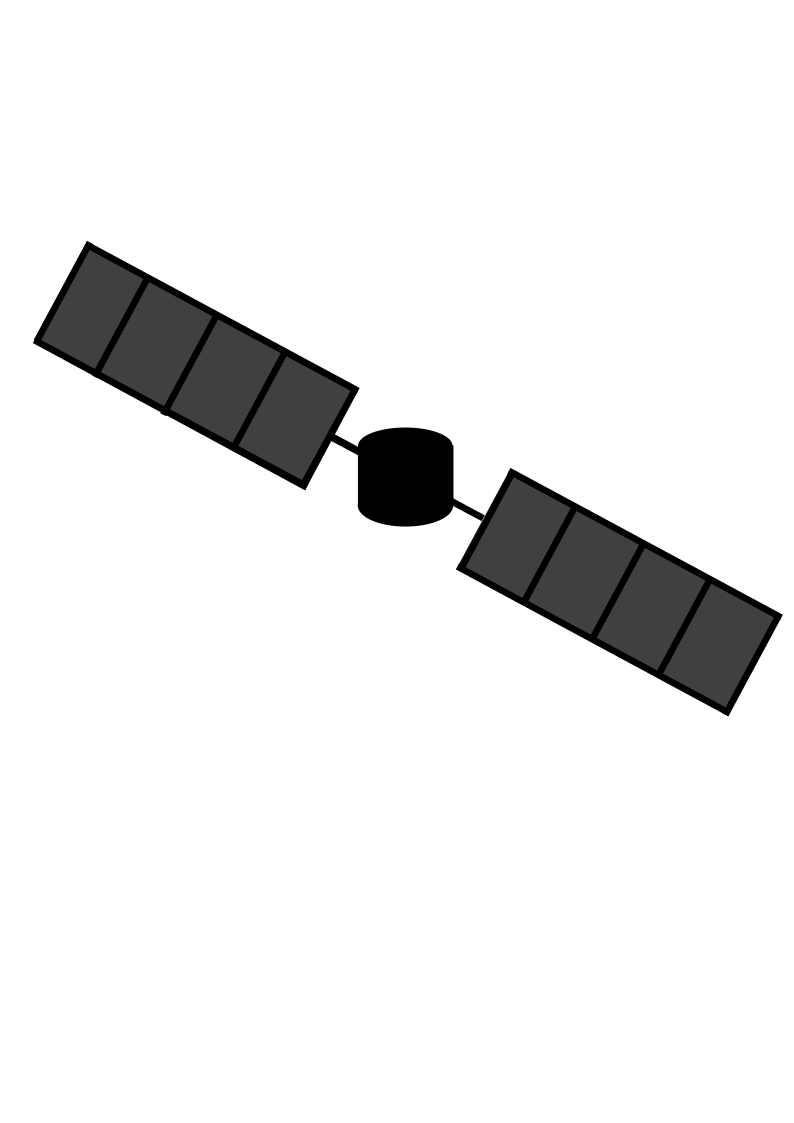
\includegraphics[width=0.25\linewidth]{figures/sat.png}};
        \node[opacity =1,inner sep=0.1pt] (russell) at (UE2)
		{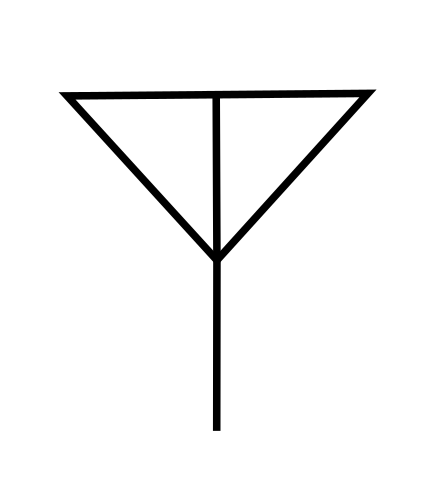
\includegraphics[width=0.05\linewidth]{figures/user_klein}};
		\node[opacity =1,inner sep=0.1pt,thick] (russell) at (UE1)
		{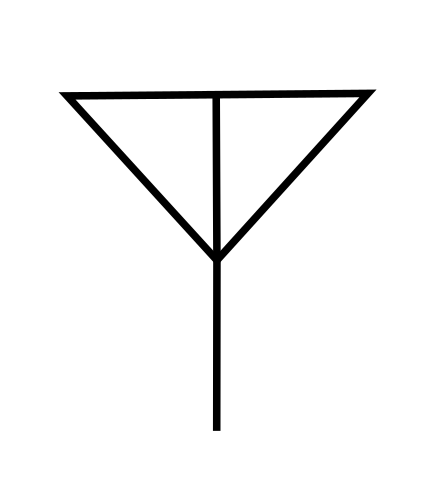
\includegraphics[width=0.05\linewidth]{figures/user_klein}};
	\end{pgfonlayer}

  	%\begin{pgfonlayer}{background}
		\node[opacity =0.3,inner sep=0.1pt] (russell) at (UE2error)
		{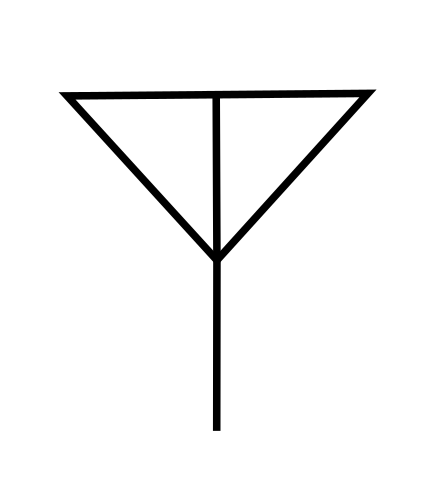
\includegraphics[width=0.05\linewidth]{figures/user_klein}};
	%\end{pgfonlayer}
 
    %\begin{pgfonlayer}{background}
		\node[opacity =0.3,inner sep=0.1pt,thick] (russell) at (UE1error)
		{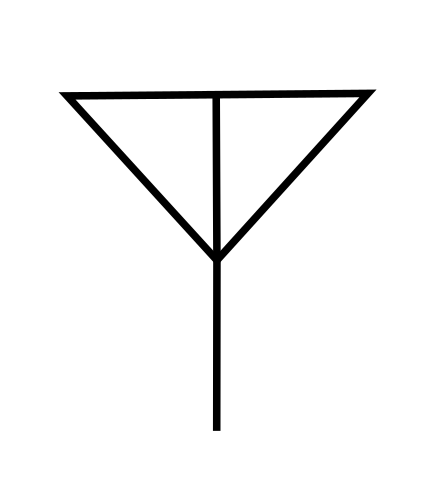
\includegraphics[width=0.05\linewidth]{figures/user_klein}};
	%\end{pgfonlayer}


	% \includegraphics[angle=90,origin=c]{file}

\end{tikzpicture}
